\chapter{Conclusioni}
Arrivati a questo punto si pu\'o confermare la versatilit\'a di {\em openHAB} al dialogo con qualsiasi tipo di dispositivo. Con lo sviluppo del sistema IOT e il collegamento di esso al software per la domotica si \'e riuscito a controllare l'irrigazione di un piccolo vaso di basilico. Esso quindi pu\'o essere tranquillamente gestito dal computer o dal proprio smartphone abilitando la modalit\'a automatica o accendendo e spegnendo manualmente la pompa dell'acqua. Inoltre \'e possibile anche visualizzare i vari stati relativi al sensore di umidit\'a e alla pompa dell'acqua. Possono essere visualizzati i risultati del lavoro alle Figure \ref{fig:smart_garden_1}, \ref{fig:smart_garden_2}, \ref{fig:smart_garden_3}, \ref{fig:smart_garden_4}.

\begin{figure}
    \centering
    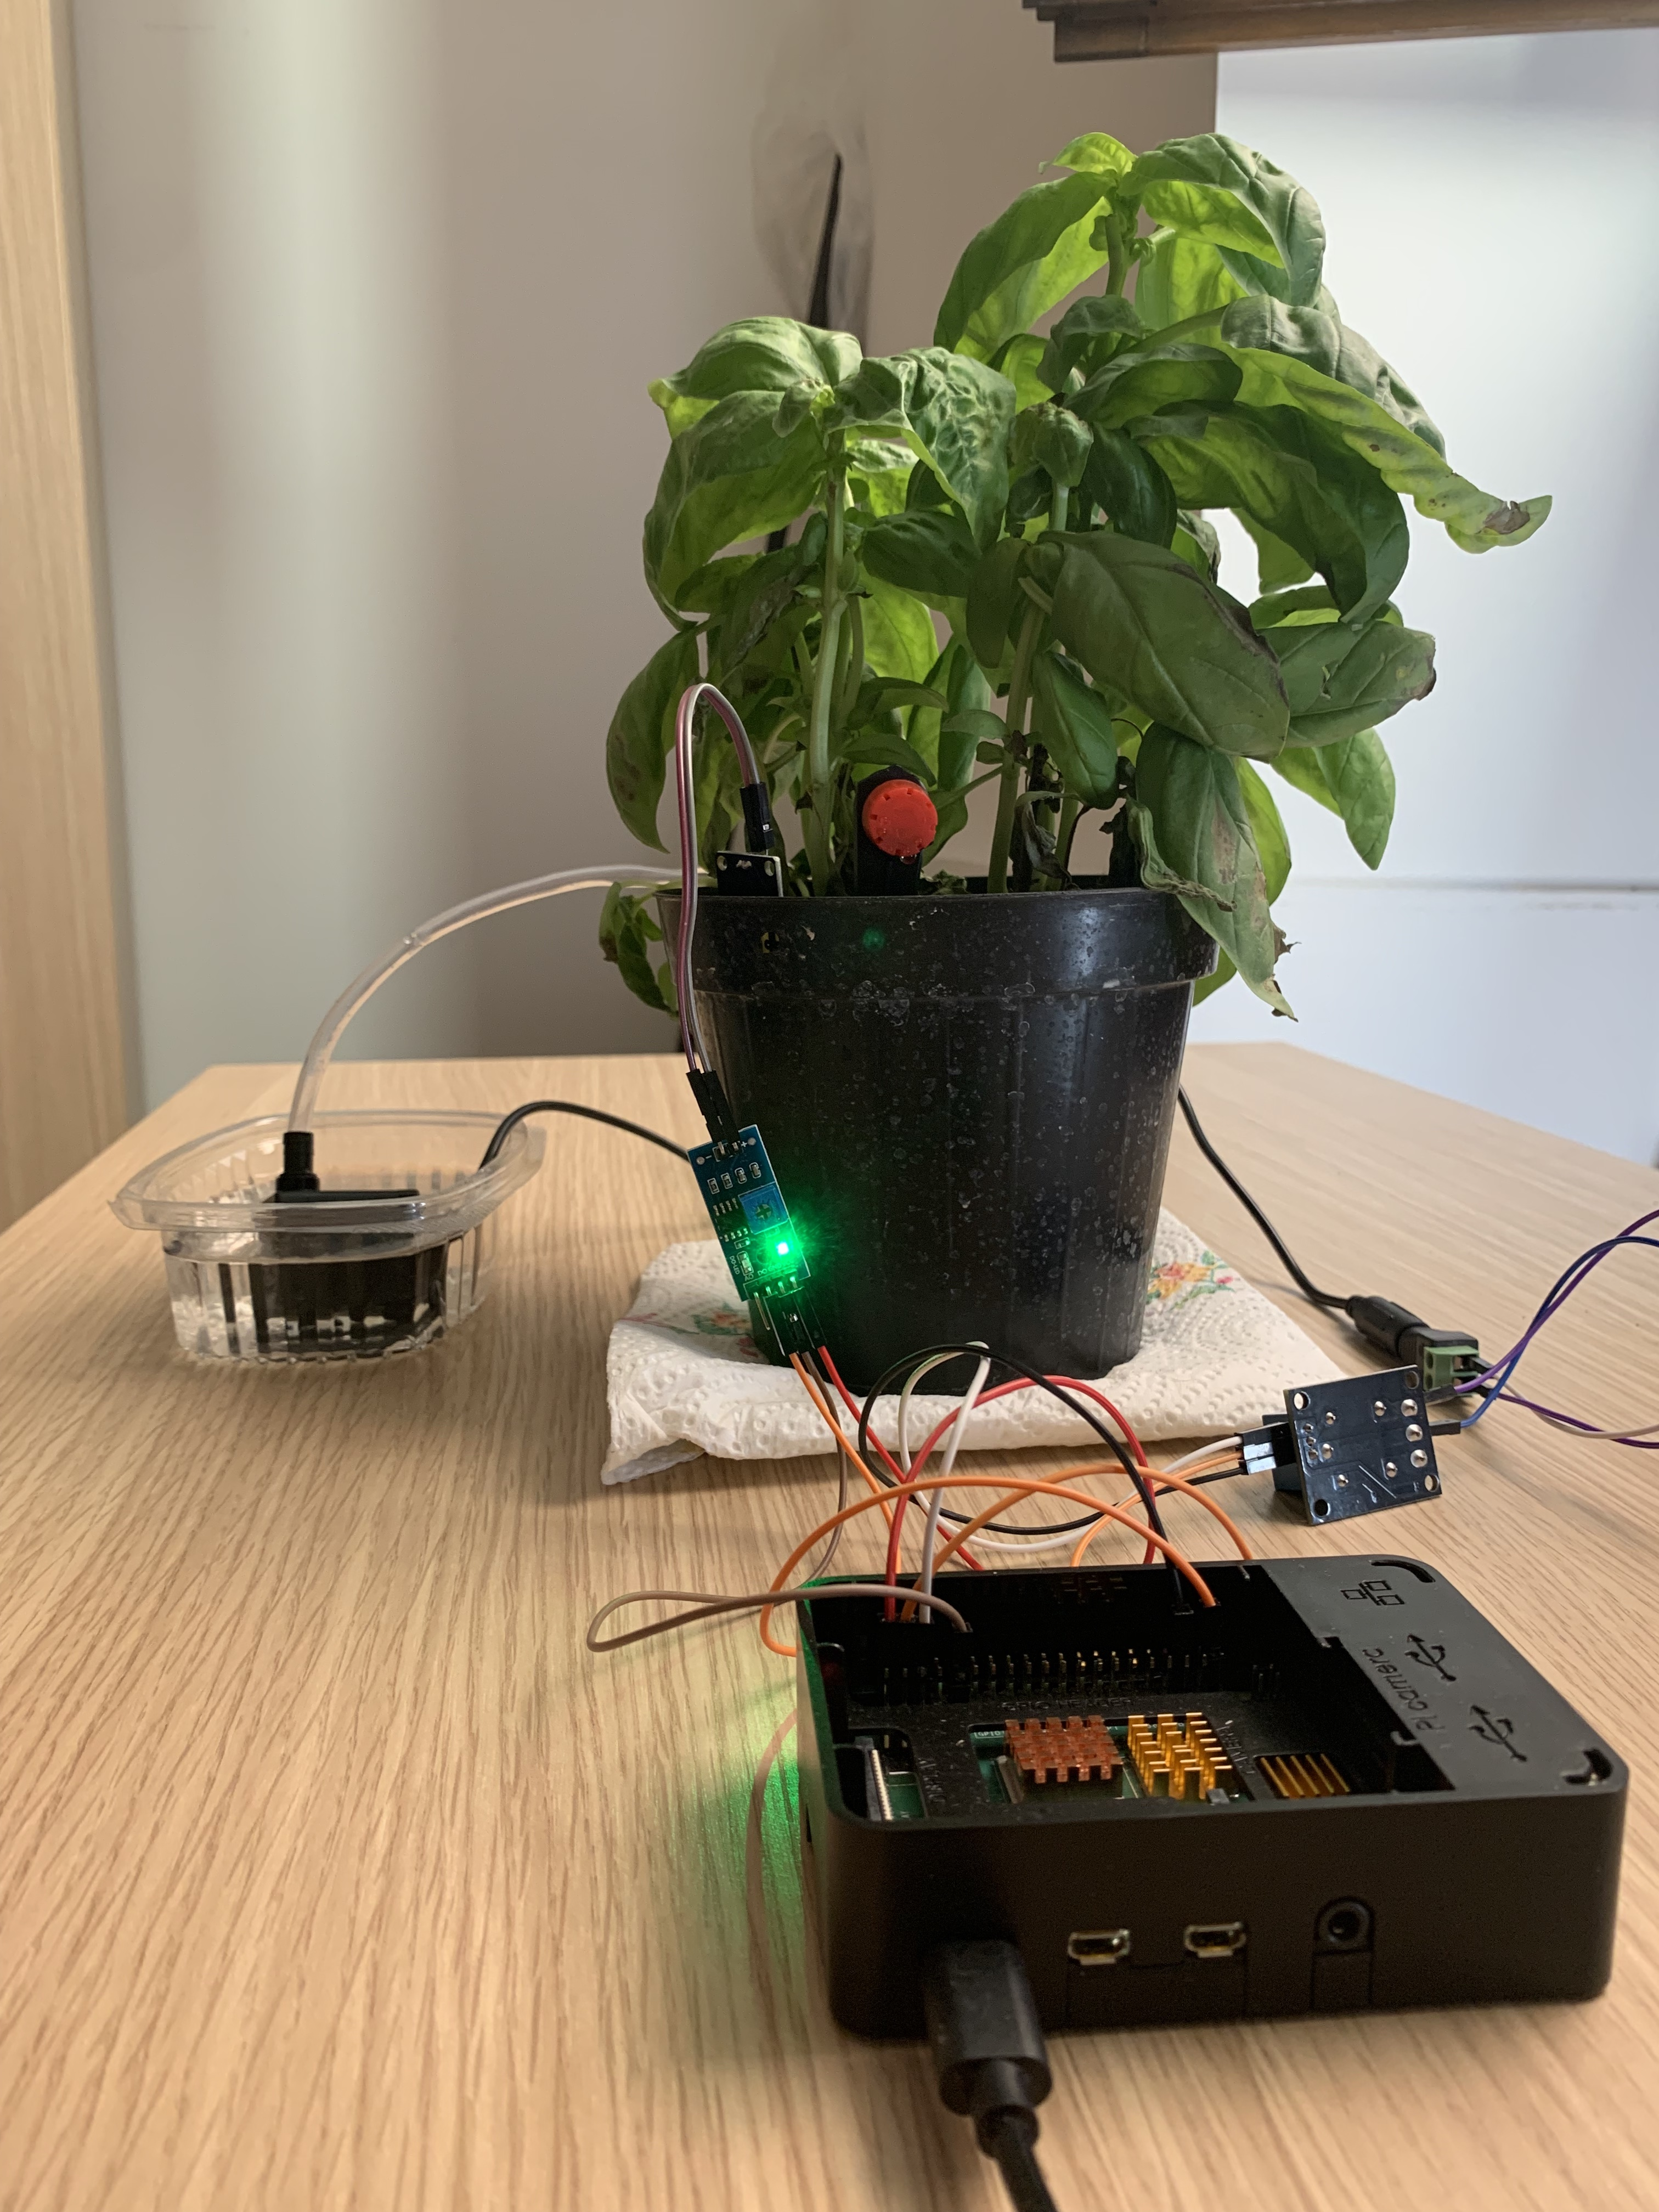
\includegraphics[width=12cm]{Immagini/smart_garden_1}
    \caption{Smart Garden di fianco}
    \label{fig:smart_garden_1}
\end{figure}

\begin{figure}
    \centering
    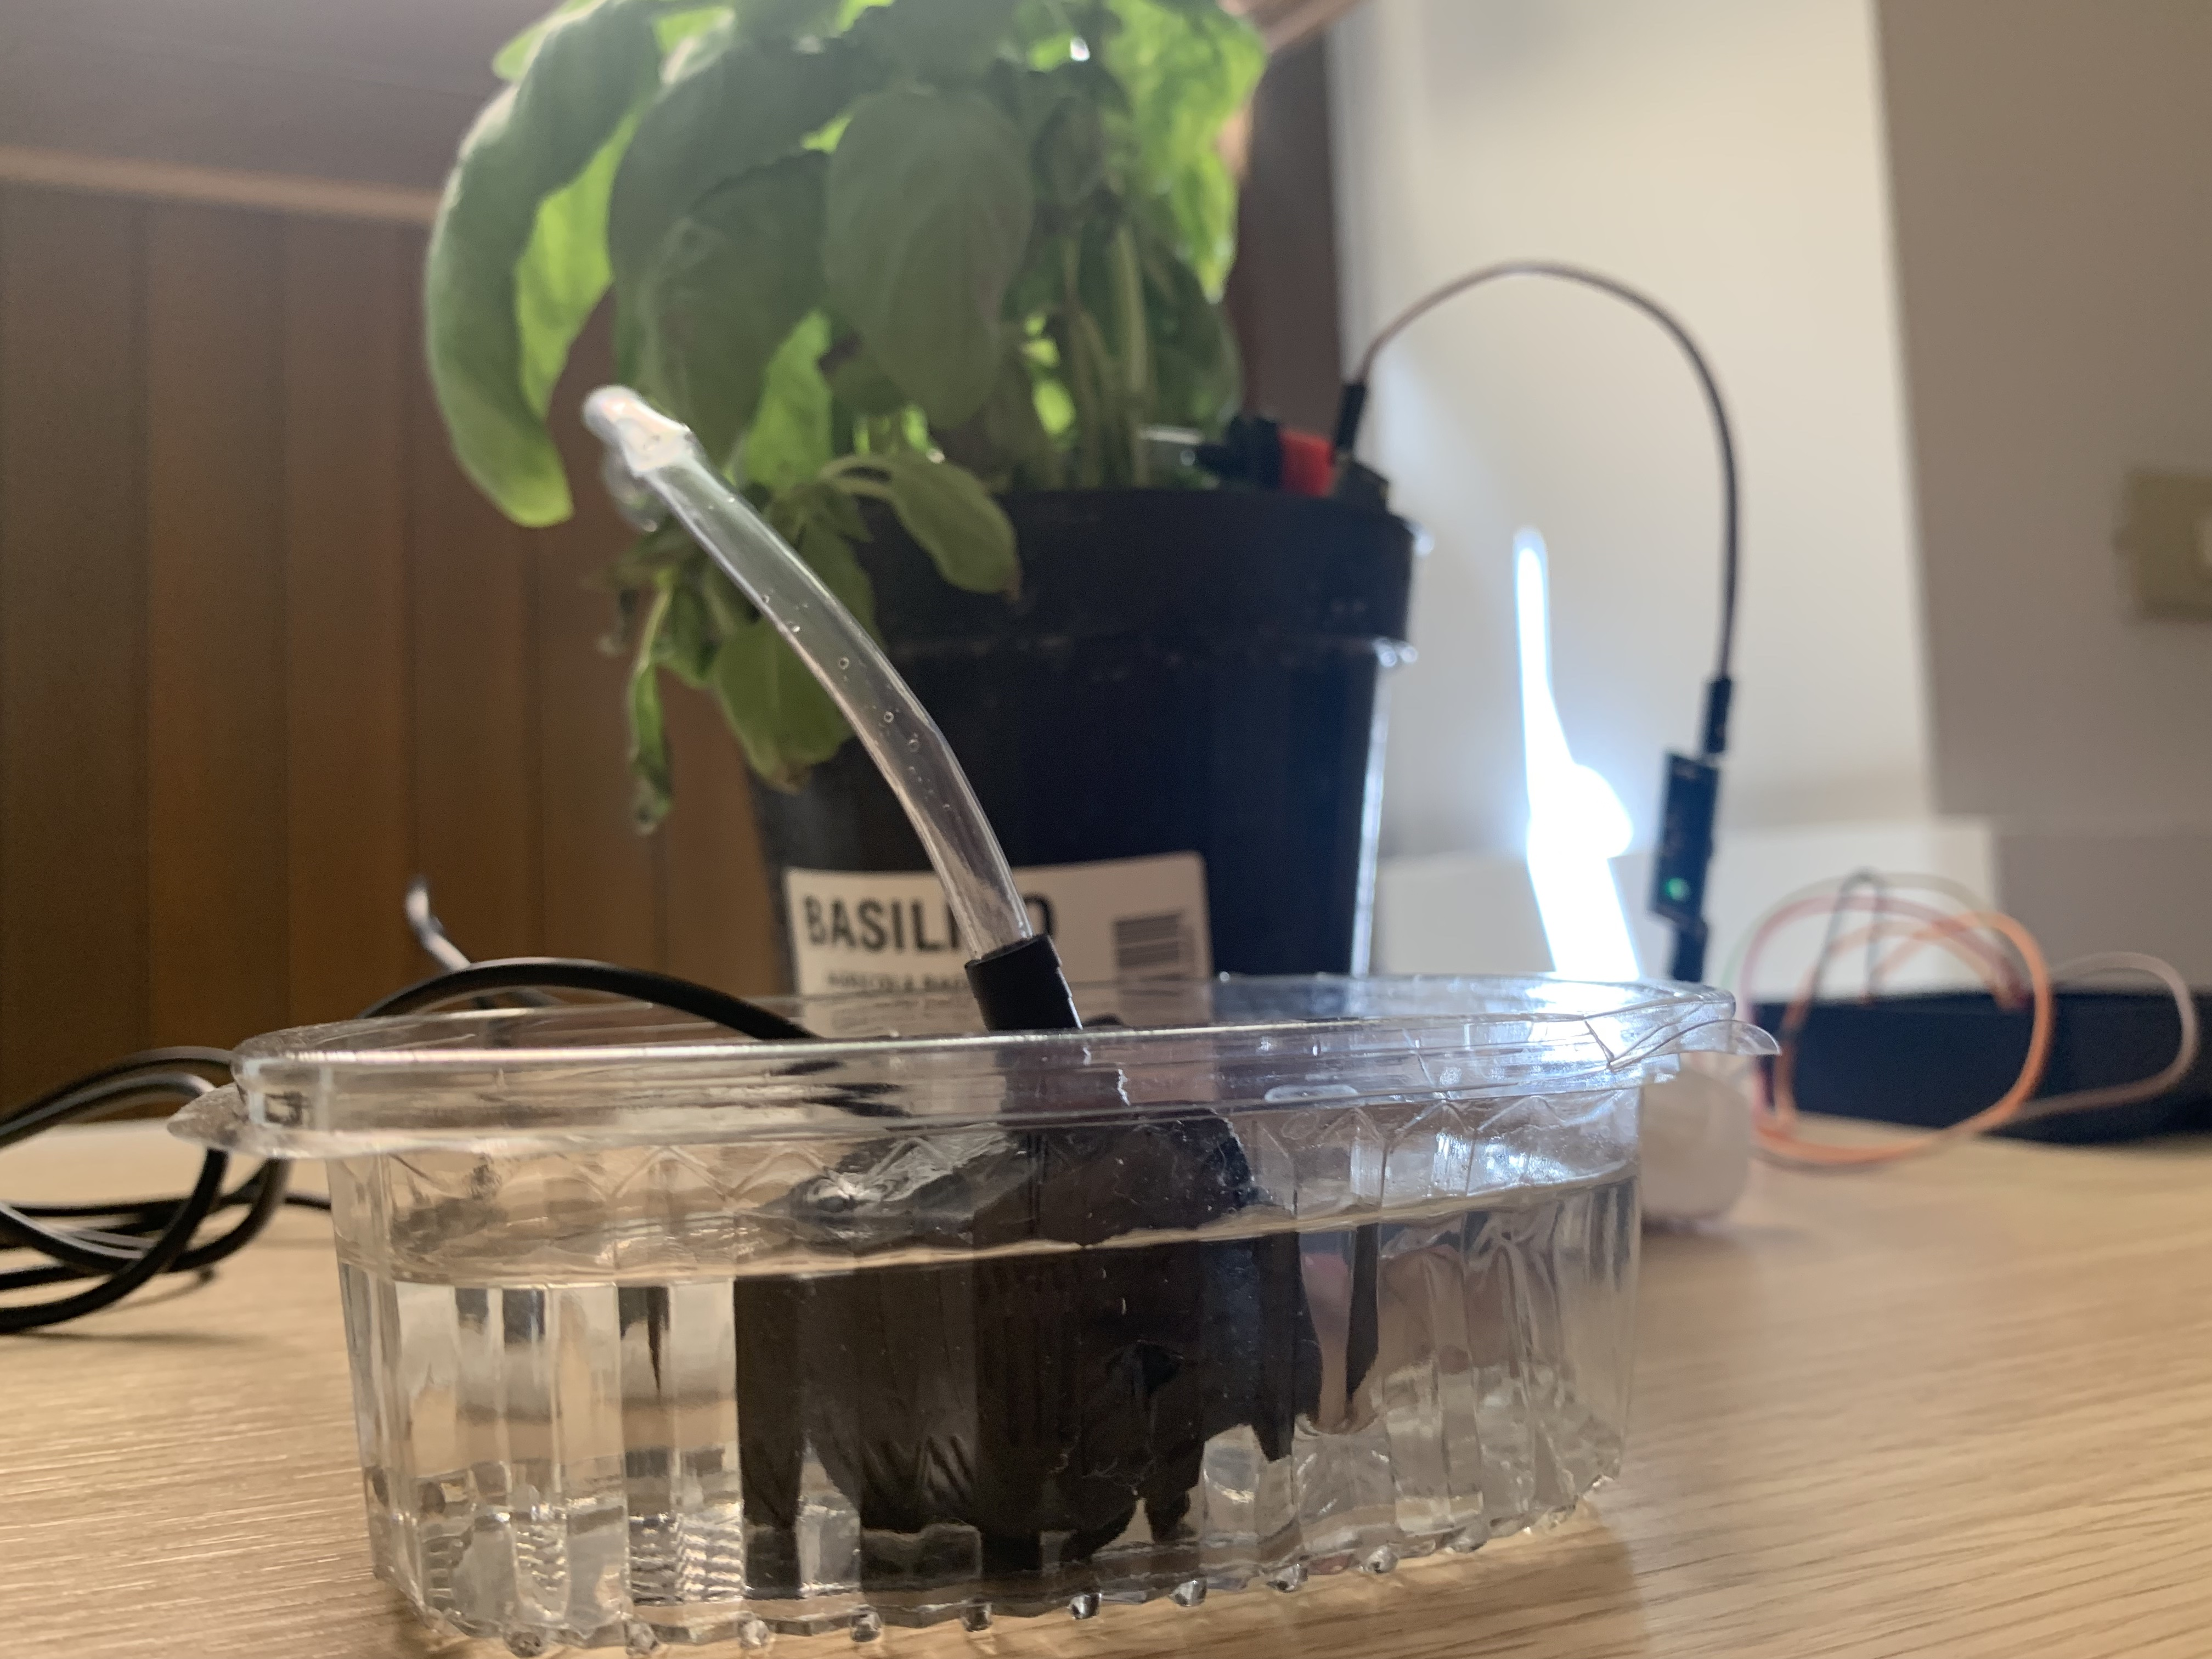
\includegraphics[width=12cm]{Immagini/smart_garden_2}
    \caption{Smart Garden pompa dell'acqua}
    \label{fig:smart_garden_2}
\end{figure}

\begin{figure}
    \centering
    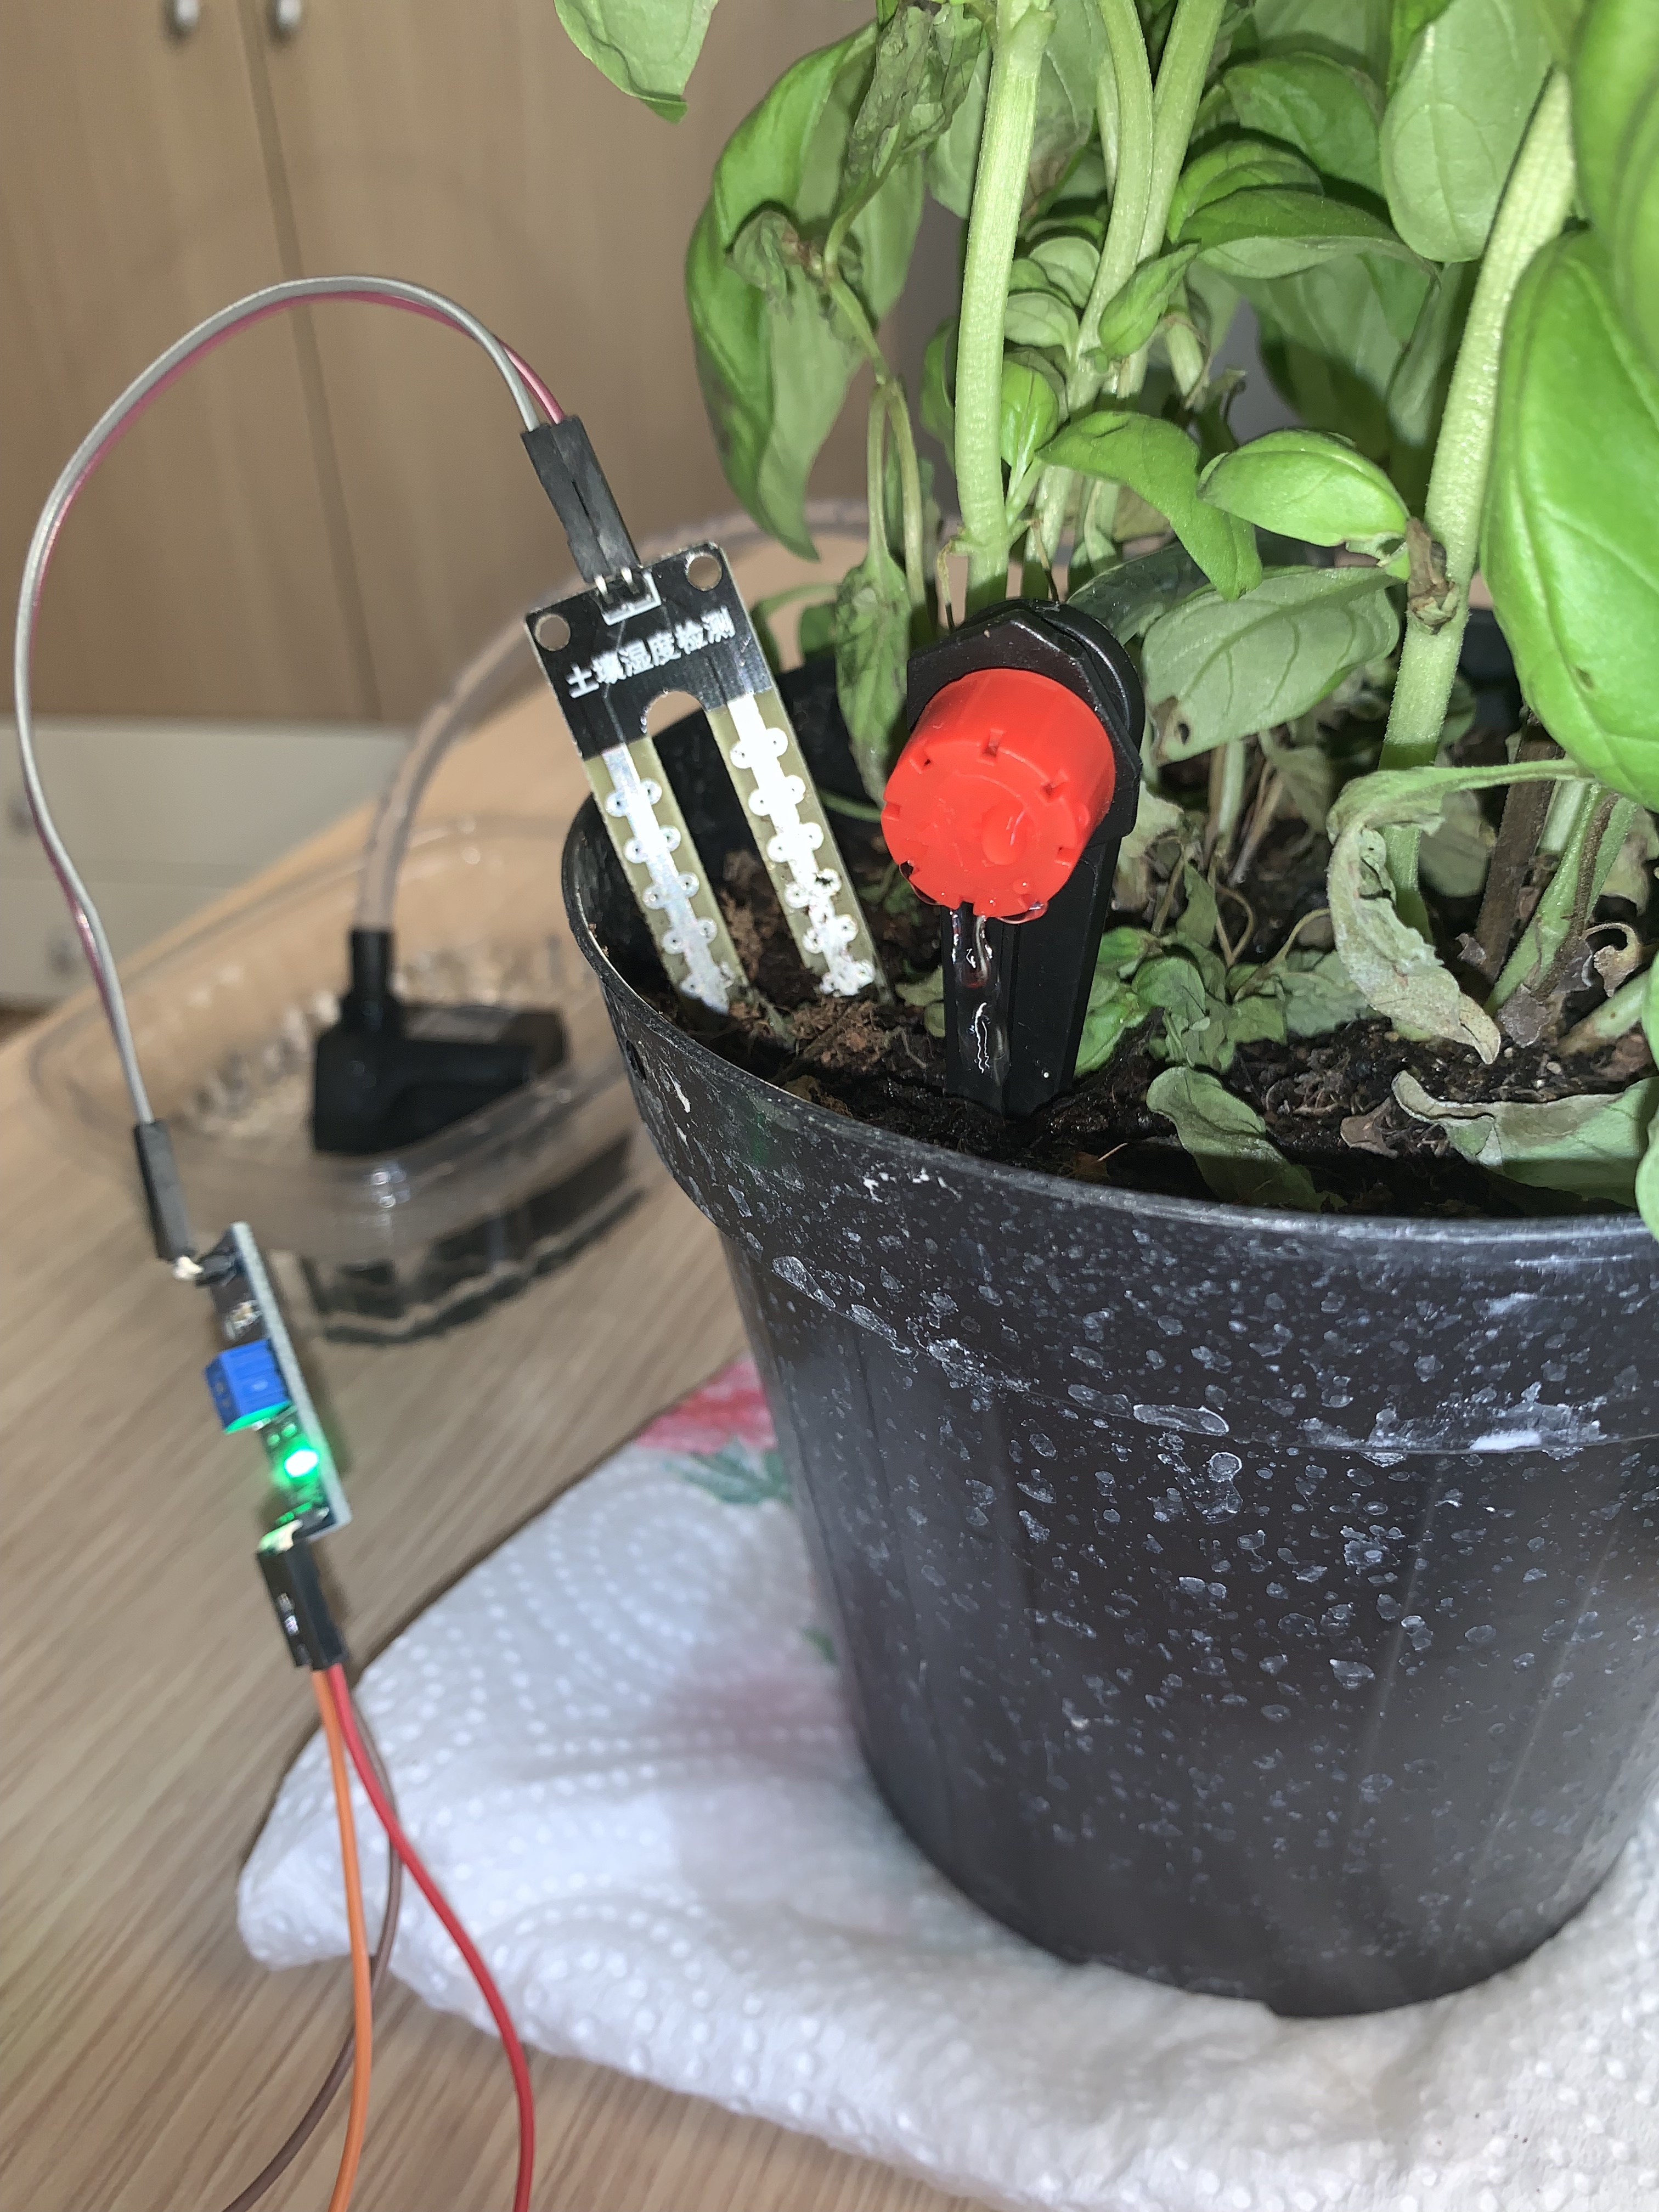
\includegraphics[width=12cm]{Immagini/smart_garden_3}
    \caption{Smart Garden sensore di umidit\'a e erogazione dell'acqua}
    \label{fig:smart_garden_3}
\end{figure}

\begin{figure}
    \centering
    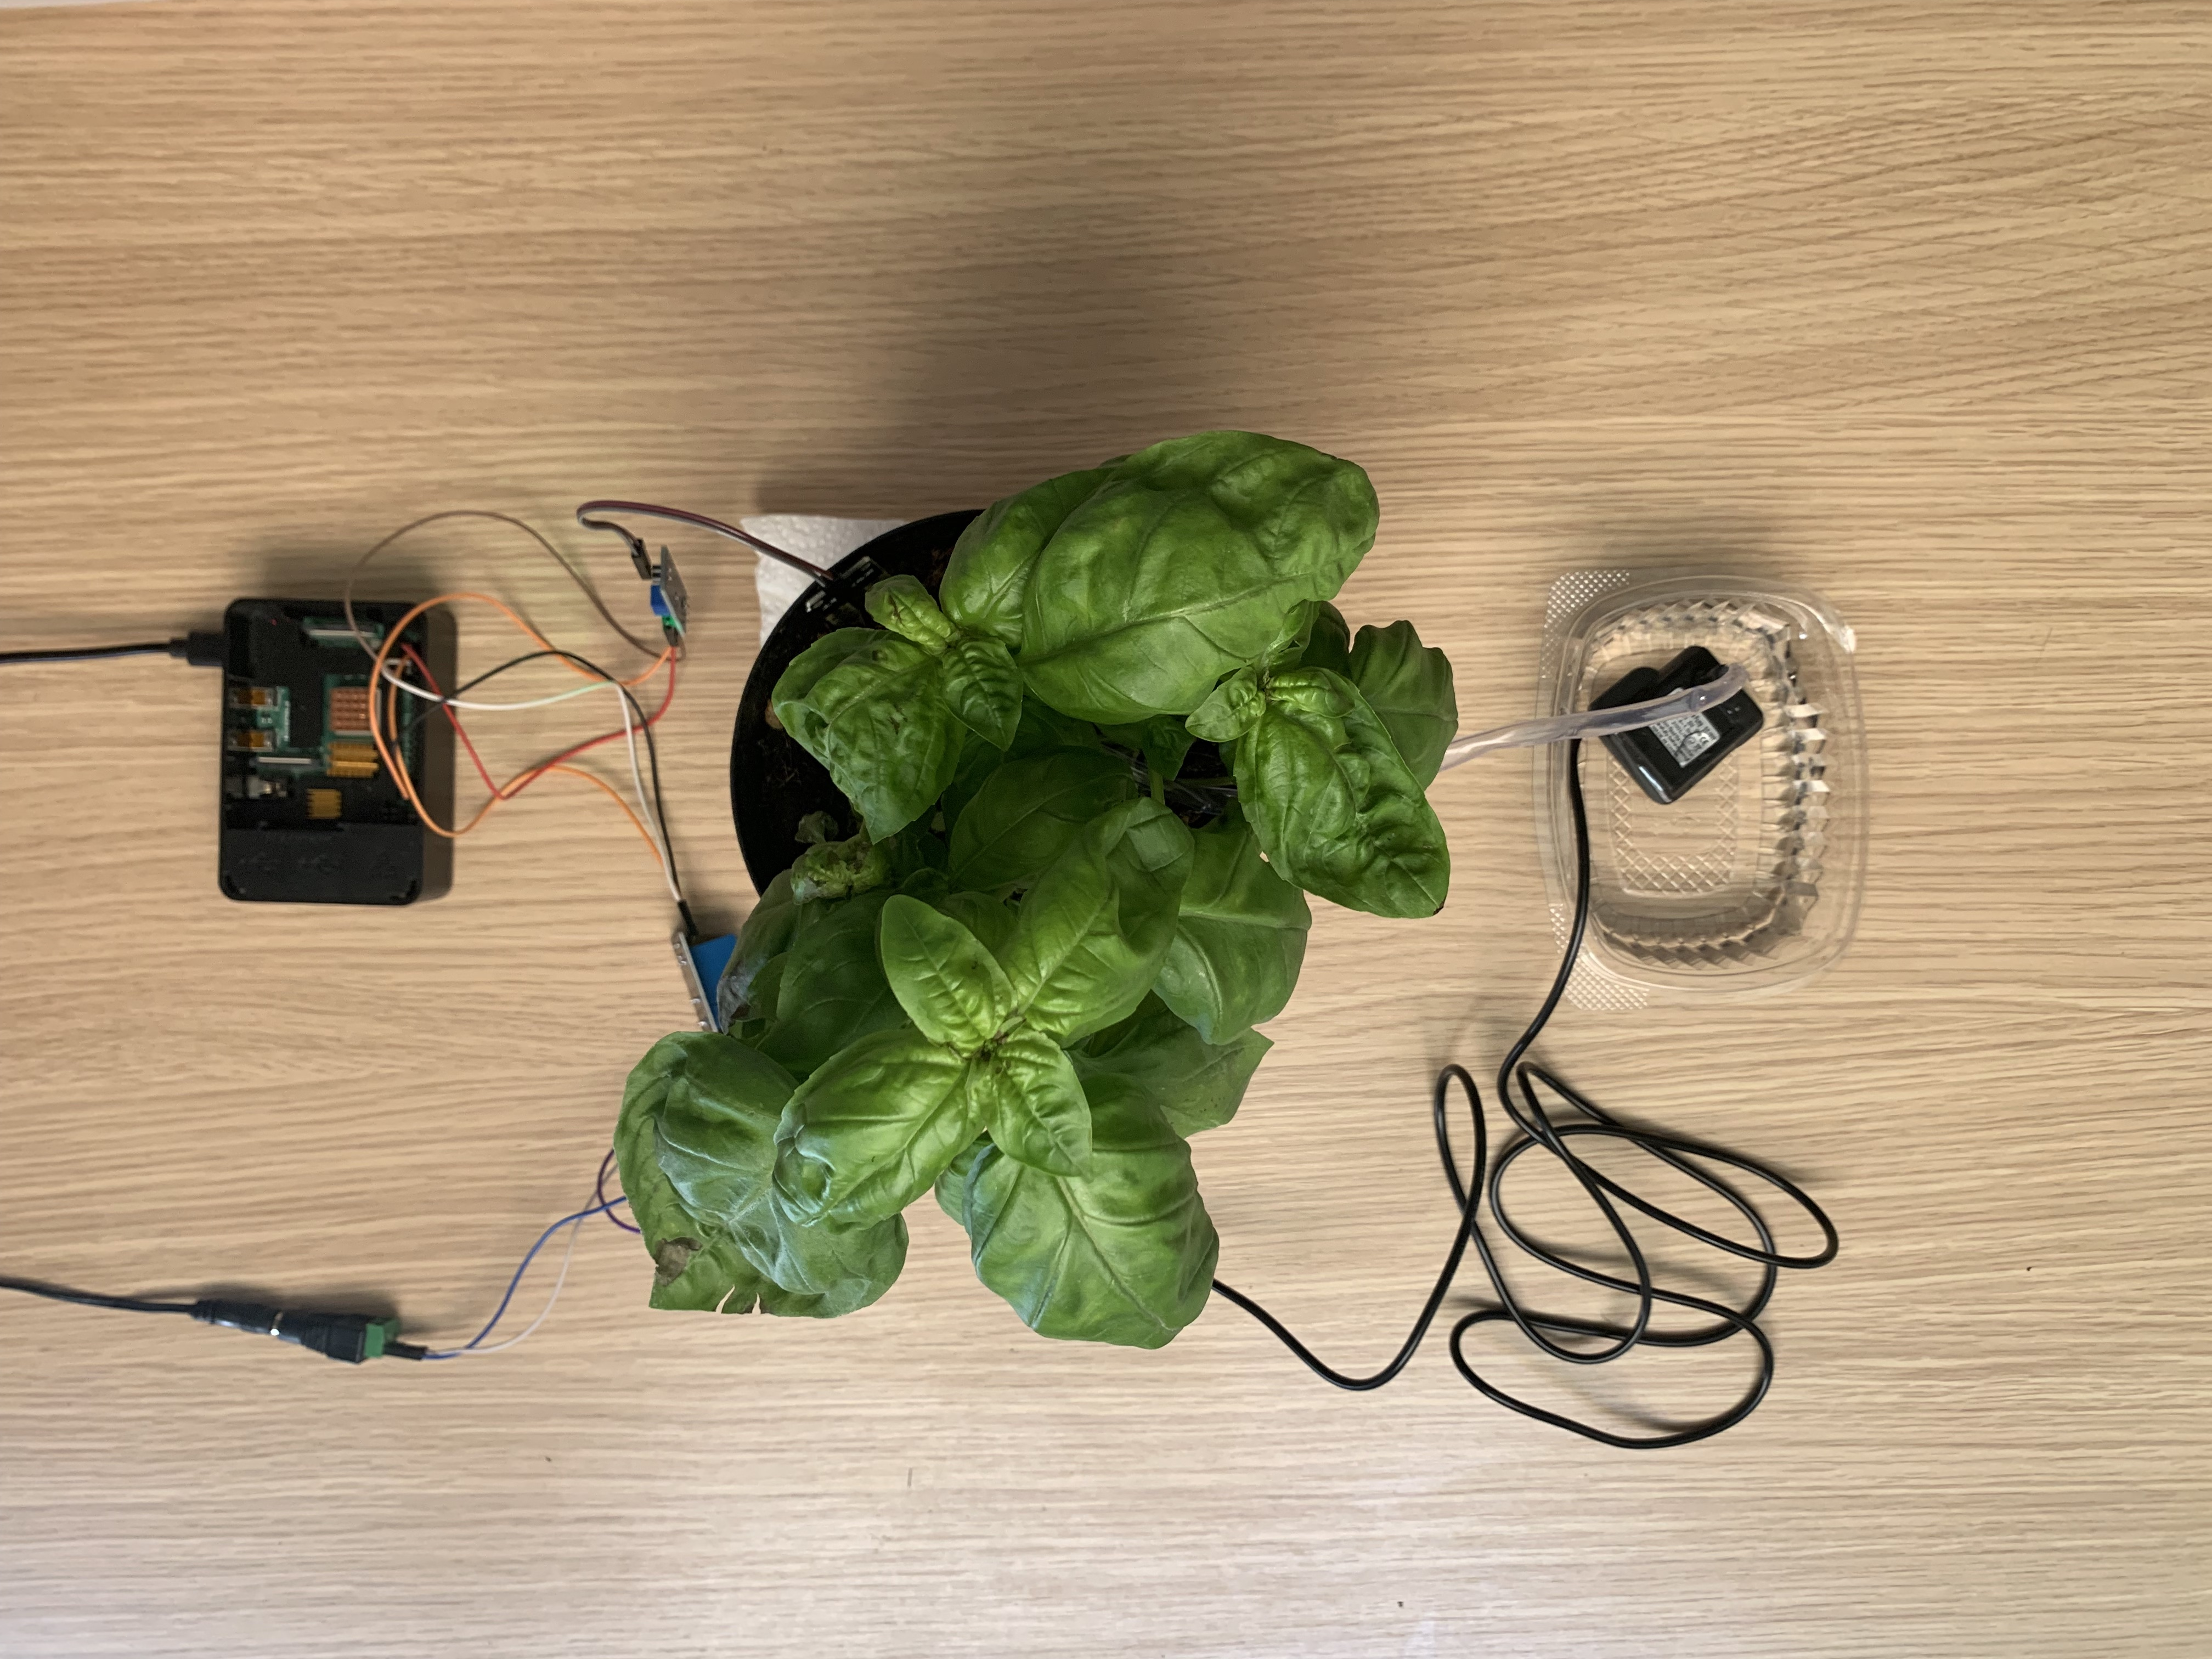
\includegraphics[width=12cm]{Immagini/smart_garden_4}
    \caption{Smart Garden dall'alto}
    \label{fig:smart_garden_4}
\end{figure}